\documentclass[aspectratio=1610]{beamer}

\title{Wildcat Beamer Theme}
\date{April 2026}
\author{Aaron Wolf (Northwestern University)}

% Theme options — combine any of these in a single \usetheme call:
%   \usetheme[
%     pattern=triangle,
%     color=nudarkblue,
%     font=poppins,
%     numbering=progressbar,
%     sectionpage=on,
%     agendastyle=pattern
%   ]{wildcat}
%
% pattern: facet (default), facetrand, triangle, triangleiso, trianglemesh,
%          squares, circles, hexraise, hexrand, network, quilt, plain
% color: any named color (nu* colors are all available after theme loads).
%        All wcprimary shades are auto-generated. Omit to keep NU purple.
% font: noto (Noto Sans), poppins (Poppins+IBM Plex), nu (Campton+Akkurat),
%        installed (system fonts), or omit for default (Fira Sans — no files needed)
% numbering: fraction (default), number, progressbar, none
% sectionpage: on (default) or none
% agendastyle: plain (default) or pattern
% breadcrumb: on or none (default)
\usetheme{wildcat}

% You change the titlegraphic to whatever you want, or comment it out to remove it.
\titlegraphic{
\includegraphics[scale=0.25]{logo-northwestern.pdf}}

% % For fine-grained control over shades, override colors manually AFTER \usetheme.
% % For example, Yale Blue (#00356b) with hand-tuned shades:
% \definecolor{wcprimary}{RGB}{0,53,107}
% \definecolor{wcprimary140}{RGB}{0, 34, 70}
% \definecolor{wcprimary130}{RGB}{0, 40, 80}
% \definecolor{wcprimary120}{RGB}{0, 45, 91}
% \definecolor{wcprimary110}{RGB}{0, 50, 102}
% \definecolor{wcprimary40}{RGB}{153, 174, 196}
% \definecolor{wcprimary30}{RGB}{179, 194, 211}
% \definecolor{wcprimary20}{RGB}{204, 215, 225}
% \definecolor{wcprimary10}{RGB}{230, 235, 240}

% % Alert and example colors:
% \definecolor{wcalerted}{RGB}{189,83,25}
% \definecolor{wcexample}{RGB}{95,113,45}

% % If you want to change the general slide background color), 
% % you can use the following command:
%\setbeamercolor{background canvas}{bg=nupurple10!30}

% % Turn off section slides (pass sectionpage=none to \usetheme)
% \usetheme[sectionpage=none]{wildcat}

% % Use a custom background pattern 
% % (see bg-gallery/bg-template.tex for an example 
% % of how to define your own pattern):
% % bg-template.tex — Community pattern template for the Wildcat Beamer theme
%
% HOW TO USE
% ----------
% Add this line to your preamble, AFTER \usetheme{wildcat} (adjust the path
% and filename as needed):
%
%   % bg-template.tex — Community pattern template for the Wildcat Beamer theme
%
% HOW TO USE
% ----------
% Add this line to your preamble, AFTER \usetheme{wildcat} (adjust the path
% and filename as needed):
%
%   % bg-template.tex — Community pattern template for the Wildcat Beamer theme
%
% HOW TO USE
% ----------
% Add this line to your preamble, AFTER \usetheme{wildcat} (adjust the path
% and filename as needed):
%
%   \input{bg-gallery/bg-template} 
%
% Note: use \input{}, not \include{}. The \include command only works inside
% the document body; pattern commands must be set in the preamble so that
% the theme's background saveboxes are populated with the correct pattern.
%
%
% HOW TO CONTRIBUTE A PATTERN
% ----------------------------
% 1. Copy this file and give it a descriptive name (e.g. bg-chevron.tex).
% 2. Rename \bgpatterntemplate to something unique (e.g. \bgpatternchevron).
% 3. Replace the TikZ drawing commands in \bgpatterntemplate with your own.
%    The command receives one argument (#1) — the color — so the theme can
%    reuse it in different contexts (title, section slides, tcolorbox blocks).
%    Your drawing should fill the full slide; the enclosing tikzpicture
%    bounding box is already set to (0,0)--(\paperwidth,\paperheight).
% 4. Submit a pull request to https://github.com/aarondwolf/wildcat
%
%
% PATTERN COMMAND REQUIREMENTS
% -----------------------------
% \bgpatterntemplate{color}  — draws a full-slide background given a color name.
%   - Must work inside an existing tikzpicture (no \begin{tikzpicture} wrapper).
%   - The bounding box already covers the full slide; just draw your shapes.
%   - Use #1 as the color argument wherever you reference the theme color.
%   - Lighter/darker shades (#1!30!white, #1!80!black, etc.) are fine to use.
%
% -----------------------------------------------------------------------
% EXAMPLE PATTERN: plain solid fill
% -----------------------------------------------------------------------
% This is the simplest possible pattern — a single solid rectangle covering
% the entire slide. Replace the \fill command below with your own TikZ
% drawing to create a new pattern.

\newcommand{\bgpatterntemplate}[1]{%
  \fill[#1] (0,0) rectangle (\paperwidth,\paperheight);%
  % Add your Tikz commands here. For color mising, use
  % the pattern #1!N!<colorname>, where N is a number
  % from 0 to 100 indicating the percentage of mixing. 
  % For example:
  %   #1!30!white — 30% white, 70% base color
  %   #1!80!black — 80% black, 20% base color
}

% Wire the pattern into the theme. Both lines are required:
%   \bgpattern      — used for the title page, section slides, and standout frames
%   \bgpatternblock — used for pblock/palertblock/pexampleblock title bars
%                     (receives the block color as its argument)
\renewcommand{\bgpattern}{\bgpatterntemplate{wcprimary}}
\renewcommand{\bgpatternblock}[1]{\bgpatterntemplate{#1}}
 
%
% Note: use \input{}, not \include{}. The \include command only works inside
% the document body; pattern commands must be set in the preamble so that
% the theme's background saveboxes are populated with the correct pattern.
%
%
% HOW TO CONTRIBUTE A PATTERN
% ----------------------------
% 1. Copy this file and give it a descriptive name (e.g. bg-chevron.tex).
% 2. Rename \bgpatterntemplate to something unique (e.g. \bgpatternchevron).
% 3. Replace the TikZ drawing commands in \bgpatterntemplate with your own.
%    The command receives one argument (#1) — the color — so the theme can
%    reuse it in different contexts (title, section slides, tcolorbox blocks).
%    Your drawing should fill the full slide; the enclosing tikzpicture
%    bounding box is already set to (0,0)--(\paperwidth,\paperheight).
% 4. Submit a pull request to https://github.com/aarondwolf/wildcat
%
%
% PATTERN COMMAND REQUIREMENTS
% -----------------------------
% \bgpatterntemplate{color}  — draws a full-slide background given a color name.
%   - Must work inside an existing tikzpicture (no \begin{tikzpicture} wrapper).
%   - The bounding box already covers the full slide; just draw your shapes.
%   - Use #1 as the color argument wherever you reference the theme color.
%   - Lighter/darker shades (#1!30!white, #1!80!black, etc.) are fine to use.
%
% -----------------------------------------------------------------------
% EXAMPLE PATTERN: plain solid fill
% -----------------------------------------------------------------------
% This is the simplest possible pattern — a single solid rectangle covering
% the entire slide. Replace the \fill command below with your own TikZ
% drawing to create a new pattern.

\newcommand{\bgpatterntemplate}[1]{%
  \fill[#1] (0,0) rectangle (\paperwidth,\paperheight);%
  % Add your Tikz commands here. For color mising, use
  % the pattern #1!N!<colorname>, where N is a number
  % from 0 to 100 indicating the percentage of mixing. 
  % For example:
  %   #1!30!white — 30% white, 70% base color
  %   #1!80!black — 80% black, 20% base color
}

% Wire the pattern into the theme. Both lines are required:
%   \bgpattern      — used for the title page, section slides, and standout frames
%   \bgpatternblock — used for pblock/palertblock/pexampleblock title bars
%                     (receives the block color as its argument)
\renewcommand{\bgpattern}{\bgpatterntemplate{wcprimary}}
\renewcommand{\bgpatternblock}[1]{\bgpatterntemplate{#1}}
 
%
% Note: use \input{}, not \include{}. The \include command only works inside
% the document body; pattern commands must be set in the preamble so that
% the theme's background saveboxes are populated with the correct pattern.
%
%
% HOW TO CONTRIBUTE A PATTERN
% ----------------------------
% 1. Copy this file and give it a descriptive name (e.g. bg-chevron.tex).
% 2. Rename \bgpatterntemplate to something unique (e.g. \bgpatternchevron).
% 3. Replace the TikZ drawing commands in \bgpatterntemplate with your own.
%    The command receives one argument (#1) — the color — so the theme can
%    reuse it in different contexts (title, section slides, tcolorbox blocks).
%    Your drawing should fill the full slide; the enclosing tikzpicture
%    bounding box is already set to (0,0)--(\paperwidth,\paperheight).
% 4. Submit a pull request to https://github.com/aarondwolf/wildcat
%
%
% PATTERN COMMAND REQUIREMENTS
% -----------------------------
% \bgpatterntemplate{color}  — draws a full-slide background given a color name.
%   - Must work inside an existing tikzpicture (no \begin{tikzpicture} wrapper).
%   - The bounding box already covers the full slide; just draw your shapes.
%   - Use #1 as the color argument wherever you reference the theme color.
%   - Lighter/darker shades (#1!30!white, #1!80!black, etc.) are fine to use.
%
% -----------------------------------------------------------------------
% EXAMPLE PATTERN: plain solid fill
% -----------------------------------------------------------------------
% This is the simplest possible pattern — a single solid rectangle covering
% the entire slide. Replace the \fill command below with your own TikZ
% drawing to create a new pattern.

\newcommand{\bgpatterntemplate}[1]{%
  \fill[#1] (0,0) rectangle (\paperwidth,\paperheight);%
  % Add your Tikz commands here. For color mising, use
  % the pattern #1!N!<colorname>, where N is a number
  % from 0 to 100 indicating the percentage of mixing. 
  % For example:
  %   #1!30!white — 30% white, 70% base color
  %   #1!80!black — 80% black, 20% base color
}

% Wire the pattern into the theme. Both lines are required:
%   \bgpattern      — used for the title page, section slides, and standout frames
%   \bgpatternblock — used for pblock/palertblock/pexampleblock title bars
%                     (receives the block color as its argument)
\renewcommand{\bgpattern}{\bgpatterntemplate{wcprimary}}
\renewcommand{\bgpatternblock}[1]{\bgpatterntemplate{#1}}


\begin{document}

\begin{frame}
\titlepage
\end{frame}

\begin{frame}{Introduction}
    The Wildcat theme is a Beamer theme for Northwestern University that can be easily customized with different colors, fonts, and background patterns.
    \\ ~ \\
    It is inspired by the \href{https://github.com/matze/mtheme}{Metropolis theme} by Matthias Vogelgesang, and incorporates the Northwestern University facet design pattern. Licensed under the GNU GENERAL PUBLIC LICENSE.
\end{frame}

\begin{frame}[plain]
    \tableofcontents
\end{frame}

\section{Background Patterns}

\begin{frame}[fragile]{Background Patterns}
    The theme ships with 12 built-in background patterns. The easiest way to switch is via a theme option:
    \scriptsize
    \begin{verbatim}
\usetheme[pattern=triangle]{wildcat}
    \end{verbatim}
    \normalsize

    Section pages automatically use the same pattern as the title page. Available pattern options:
    \begin{columns}[t]
    \column{0.5\textwidth}
    \begin{itemize}\footnotesize
        \item \texttt{facet} — NU facets (default)
        \item \texttt{facetrand} — NU facets (alternate)
        \item \texttt{triangle} — triangle mosaic
        \item \texttt{triangleiso} — isometric triangles
        \item \texttt{trianglemesh} — wireframe mesh
        \item \texttt{squares} — square grid
    \end{itemize}
    \column{0.5\textwidth}
    \begin{itemize}\footnotesize
        \item \texttt{circles} — circles
        \item \texttt{hexraise} — raised hex clusters
        \item \texttt{hexrand} — random hex shading
        \item \texttt{network} — network grid
        \item \texttt{quilt} — quilt rings
        \item \texttt{plain} — solid color
    \end{itemize}
    \end{columns}
    \vskip0.5em
    {\footnotesize See \href{https://github.com/aarondwolf/wildcat/blob/main/source/wildcat-gallery.pdf}{\texttt{wildcat-gallery.pdf}} for a visual preview of all patterns.}
\end{frame}


\section{Colors}

\begin{frame}
    \frametitle{Colors}
    The theme has a few Northwestern-specific colors defined, which you can use in your slides. These are:
    \begin{columns}
    \column{0.3\textwidth}
    \begin{itemize}
        \item[$\textcolor{nupurple}{\bullet}$] \textcolor{nupurple}{nupurple} 
        \item[$\textcolor{nupurple90}{\bullet}$] \textcolor{nupurple90}{nupurple90} 
        \item[$\textcolor{nupurple80}{\bullet}$] \textcolor{nupurple80}{nupurple80}
        \item[$\textcolor{nupurple70}{\bullet}$] \textcolor{nupurple70}{nupurple70}
        \item[$\textcolor{nupurple60}{\bullet}$] \textcolor{nupurple60}{nupurple60}
        \item[$\textcolor{nupurple50}{\bullet}$] \textcolor{nupurple50}{nupurple50}
        \item[$\textcolor{nupurple40}{\bullet}$] \textcolor{nupurple40}{nupurple40}
        \item[$\textcolor{nupurple30}{\bullet}$] \textcolor{nupurple30}{nupurple30}
        \item[$\textcolor{nupurple20}{\bullet}$] \textcolor{nupurple20}{nupurple20}
        \item[$\textcolor{nupurple10}{\bullet}$] \textcolor{nupurple10}{nupurple10}
    \end{itemize}
    \column{0.3\textwidth}
    \begin{itemize}
        \item[$\textcolor{nupurple160}{\bullet}$] \textcolor{nupurple160}{nupurple160}
        \item[$\textcolor{nupurple150}{\bullet}$] \textcolor{nupurple150}{nupurple150}
        \item[$\textcolor{nupurple140}{\bullet}$] \textcolor{nupurple140}{nupurple140}
        \item[$\textcolor{nupurple130}{\bullet}$] \textcolor{nupurple130}{nupurple130}
        \item[$\textcolor{nupurple120}{\bullet}$] \textcolor{nupurple120}{nupurple120}
        \item[$\textcolor{nupurple110}{\bullet}$] \textcolor{nupurple110}{nupurple110}
        \item[$\textcolor{nurichblack}{\bullet}$] \textcolor{nurichblack}{nurichblack}
        \item[$\textcolor{nubrightgreen}{\bullet}$] \textcolor{nubrightgreen}{nubrightgreen}
        \item[$\textcolor{nubrightteal}{\bullet}$] \textcolor{nubrightteal}{nubrightteal}
        \item[$\textcolor{nubrightblue}{\bullet}$] \textcolor{nubrightblue}{nubrightblue}
    \end{itemize}
    \column{0.3\textwidth}
    \begin{itemize}
        \item[$\textcolor{nubrightyellow}{\bullet}$] \textcolor{nubrightyellow}{nubrightyellow}
        \item[$\textcolor{nubrightorange}{\bullet}$] \textcolor{nubrightorange}{nubrightorange}
        \item[$\textcolor{nubrightred}{\bullet}$] \textcolor{nubrightred}{nubrightred}
        \item[$\textcolor{nudarkgreen}{\bullet}$] \textcolor{nudarkgreen}{nudarkgreen}
        \item[$\textcolor{nudarkteal}{\bullet}$] \textcolor{nudarkteal}{nudarkteal}
        \item[$\textcolor{nudarkblue}{\bullet}$] \textcolor{nudarkblue}{nudarkblue}
        \item[$\textcolor{nudarkyellow}{\bullet}$] \textcolor{nudarkyellow}{nudarkyellow}
        \item[$\textcolor{nudarkorange}{\bullet}$] \textcolor{nudarkorange}{nudarkorange}
        \item[$\textcolor{nudarkred}{\bullet}$] \textcolor{nudarkred}{nudarkred}
    \end{itemize}
    \end{columns}
\end{frame}

\begin{frame}[fragile]{Modifying the Primary Color}
    Pass a \texttt{color} option to \texttt{\textbackslash usetheme} — the theme auto-generates all lighter and darker shades automatically:
    \scriptsize
    \begin{verbatim}
\usetheme[color=nudarkblue]{wildcat}
    \end{verbatim}
    \normalsize
    You can combine \texttt{color} and \texttt{pattern} in a single line:
    \scriptsize
    \begin{verbatim}
\usetheme[color=nudarkblue, pattern=hexraise]{wildcat}
    \end{verbatim}
    \normalsize
    The \texttt{nu*} colors from the previous slide are all valid choices, as are the standard xcolor built-ins (\texttt{red}, \texttt{blue}, \texttt{cyan}, etc.). The alert and example colors (\texttt{wcalerted}, \texttt{wcexample}) are not affected and can be overridden separately.
\end{frame}

\begin{frame}[fragile]{Modifying the Primary Color: Custom RGB}
    The \texttt{color} option accepts any \textit{named} color — not raw RGB values. If your brand color isn't already defined, declare it first:
    \scriptsize
    \begin{verbatim}
\definecolor{myblue}{RGB}{0,53,107}
\usetheme[color=myblue]{wildcat}
    \end{verbatim}
    \normalsize
    When you pass a color via the \texttt{color} option, that color becomes available to use as \texttt{wcprimary} in your slides, and the theme auto-generates the lighter and darker shades as \texttt{wcprimary10}–\texttt{40} and \texttt{wcprimary110}–\texttt{140}, respectively. These are also available as named colors you can use in your slides, and the theme uses them internally for block backgrounds and pattern fills.
    \\ ~ \\
    The auto-generated shades follow a simple scale: \texttt{wcprimary10}–\texttt{40} mix the base color with white (lighter tints), and \texttt{wcprimary110}–\texttt{140} mix it with black (darker shades). These are sufficient for most use cases — if you need precise per-shade control, see the Advanced Customization section at the end of this document.
\end{frame}

\begin{frame}[fragile]
    \frametitle{Using Colors in Graphs}
    %You can use the colors in your graphs in Python, R, and Stata using the following commands:
    \begin{block}{Python}
        \footnotesize
        \begin{verbatim}
import matplotlib.pyplot as plt
import pandas as pd
plt.style.use('ggplot')
# Create colors
wcprimary = (78/255,42/255,132/255)
df = pd.read_stata("source/graphs/auto.dta")
plt.scatter(df["weight"], df["mpg"], color=wcprimary)
plt.xlabel("Weight")
plt.ylabel("MPG")
plt.savefig("source/graphs/plot-python.pdf")
plt.show()
        \end{verbatim}
    \end{block}
\end{frame}

\begin{frame}[fragile]
    \frametitle{Using Colors in Graphs}
    \begin{figure}
        \centering
        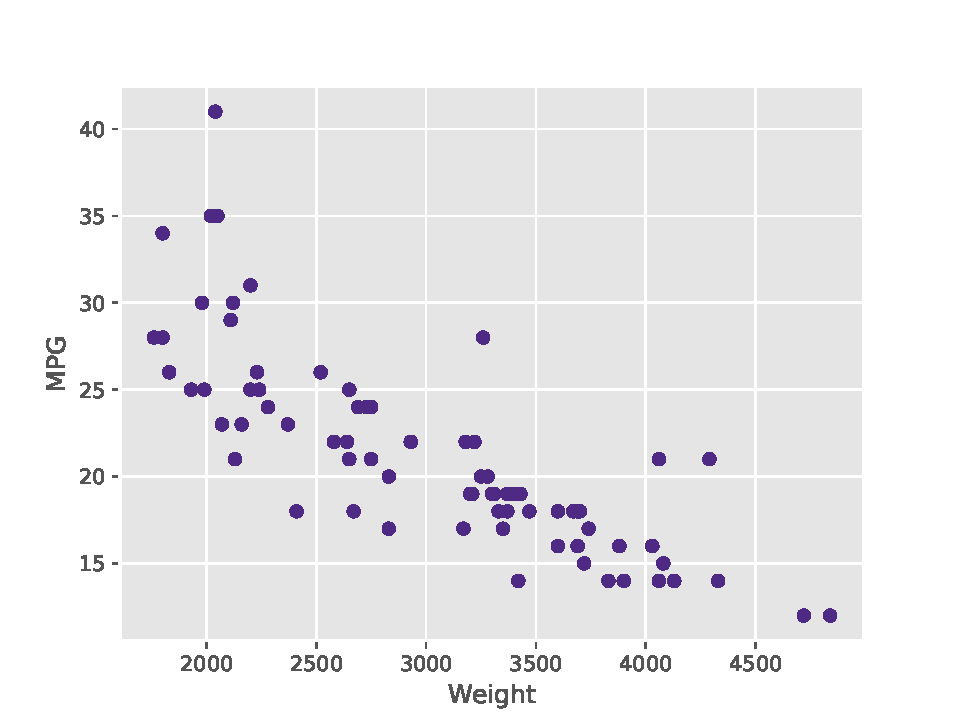
\includegraphics[width=0.62\textwidth]{graphs/plot-python.pdf}
        \caption{Python Graph Example}
        \label{fig:graph-python}
    \end{figure}
\end{frame}

\begin{frame}[fragile]
    \frametitle{Using Colors in Graphs}
    \begin{block}{R}
        \footnotesize
        \begin{verbatim}
library(ggplot2)
library(haven)
# Load data
df <- read_dta("source/graphs/auto.dta")
# Define custom RGB colors
wcprimary <- rgb(78/255, 42/255, 132/255)

# Plot mpg against weight, with marker color wcprimary
plot <- ggplot(df, aes(x = weight, y = mpg)) +
    geom_point(color = wcprimary) +
    labs(x = "Weight", y = "MPG")

# Save the plot to a file with a specific size
ggsave("source/graphs/plot-R.pdf", plot, width = 8, height = 5)
        \end{verbatim}
    \end{block}
\end{frame}



\begin{frame}[fragile]
    \frametitle{Using Colors in Graphs}
    \begin{figure}
        \centering
        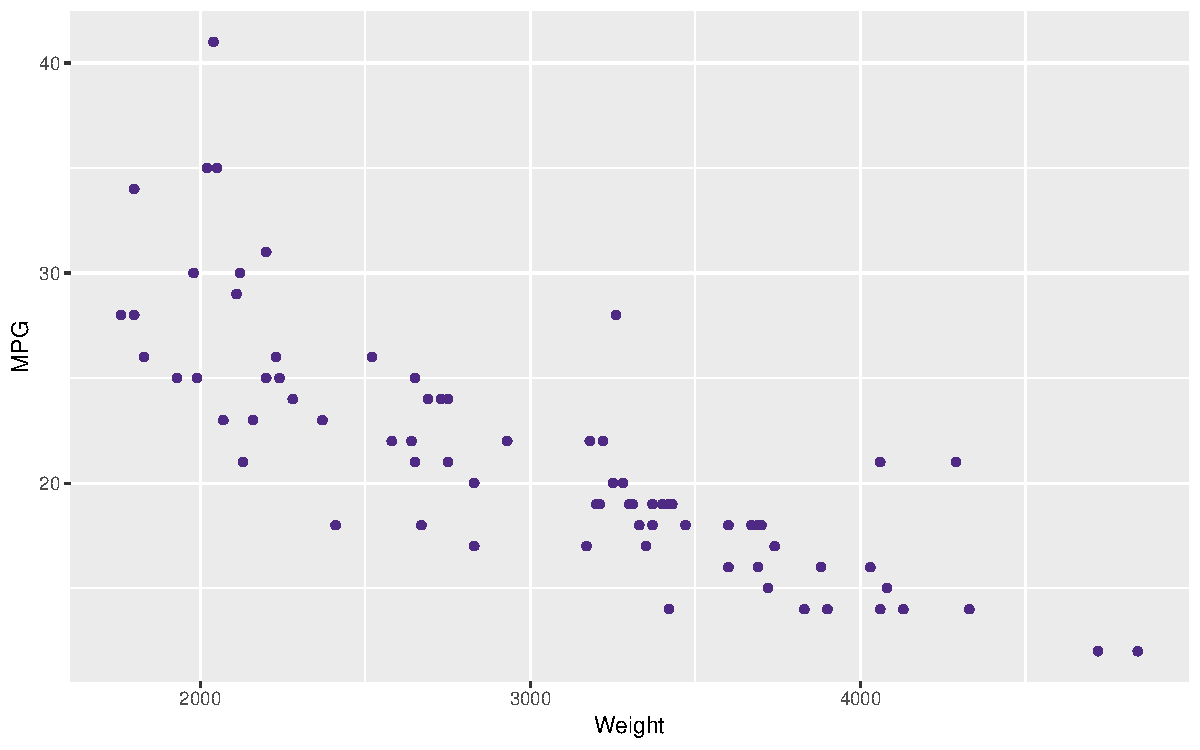
\includegraphics[width=0.7\textwidth]{graphs/plot-R.pdf}
        \caption{R Graph Example}
        \label{fig:graph-R}
    \end{figure}
\end{frame}

\begin{frame}[fragile]
    \frametitle{Using Colors in Graphs}
    \begin{block}{Stata}
        \footnotesize
        \begin{verbatim}
ssc install schemepack, replace
sysuse auto, clear
local wcprimary "78 42 132"

twoway (scatter mpg weight, mcolor("`wcprimary'")), ///
        scheme(gg_tableau)
        
graph export "source/graphs/plot-stata.pdf", replace
        \end{verbatim}
    \end{block}
\end{frame}

\begin{frame}[fragile]
    \frametitle{Using Colors in Graphs}
    \begin{figure}
        \centering
        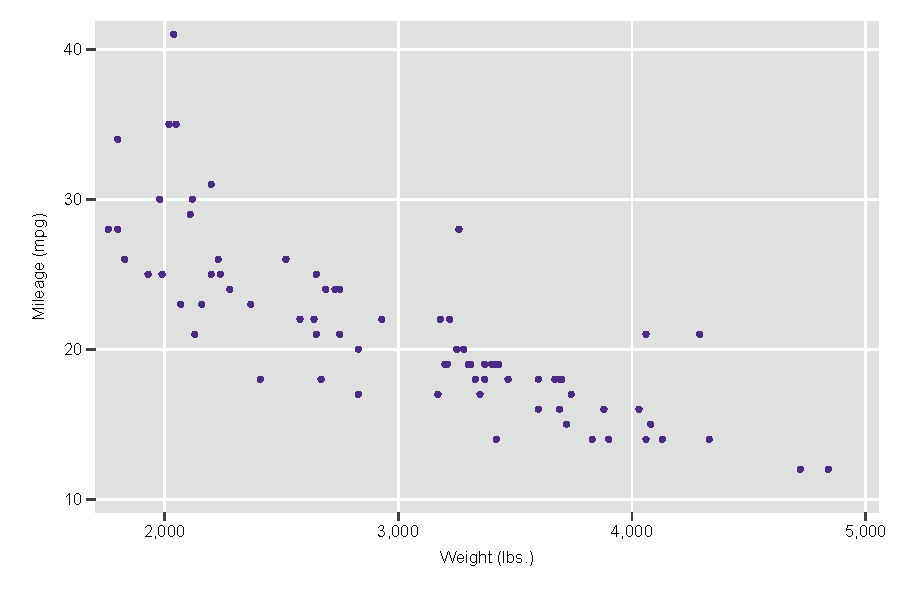
\includegraphics[width=0.7\textwidth]{graphs/plot-stata.pdf}
        \caption{Stata Graph Example}
        \label{fig:graph-stata}
    \end{figure}
\end{frame}

\section{Fonts}
\begin{frame}[fragile]{Fonts: Default (Fira Sans)}
    By default, the theme uses \textbf{Fira Sans} --- a clean, geometric sans-serif that ships with TeX Live and MiKTeX and is pre-installed on Overleaf. No font files need to be downloaded or bundled:
    \scriptsize
    \begin{verbatim}
\usetheme{wildcat}          % Fira Sans loads automatically
    \end{verbatim}
    \normalsize
    \textbf{Overleaf:} works out of the box. \\
    \textbf{MiKTeX:} auto-installs on first compile. \\
    \textbf{TeX Live:} if the font is not found, run \texttt{tlmgr install fira} in your terminal, then recompile. \\[0.5em]
    Requires \textbf{XeLaTeX} or \textbf{LuaLaTeX} — PDFLaTeX will fail.
\end{frame}

\begin{frame}[fragile]{Fonts: Noto Sans}
    For another bundled, Overleaf-friendly option, use \texttt{font=noto}. It uses \textbf{Noto Sans} and mirrors the same weight structure as the default Fira setup:
    \scriptsize
    \begin{verbatim}
\usetheme[font=noto]{wildcat}
    \end{verbatim}
    \normalsize
    This is a good default when you want broad Unicode coverage and don't want to upload font files. As with the other theme fonts, compile with \textbf{XeLaTeX} or \textbf{LuaLaTeX}.
\end{frame}

\begin{frame}[fragile]{Fonts: Poppins + IBM Plex Sans}
    For a closer match to Northwestern's recommended free fonts, use \texttt{font=poppins}. Download \href{https://fonts.google.com/specimen/Poppins}{Poppins} and \href{https://fonts.google.com/specimen/IBM+Plex+Sans}{IBM Plex Sans} from Google Fonts and place them in a \texttt{fonts/} folder next to your \texttt{.tex} file:
    \scriptsize
    \begin{verbatim}
\usetheme[font=poppins]{wildcat}
    \end{verbatim}
    \begin{verbatim}
your-presentation/
  your-slides.tex
  fonts/
    Poppins/
      Poppins-Medium.ttf    Poppins-MediumItalic.ttf
      Poppins-SemiBold.ttf  Poppins-SemiBoldItalic.ttf
      Poppins-Light.ttf     Poppins-LightItalic.ttf
      Poppins-Regular.ttf   Poppins-Italic.ttf
    IBM_Plex_Sans/
      IBMPlexSans-Light.ttf      IBMPlexSans-LightItalic.ttf
      IBMPlexSans-Regular.ttf    IBMPlexSans-Italic.ttf
    \end{verbatim}
    \normalsize
    For proprietary Northwestern brand fonts (Campton + Akkurat Pro), see the Advanced Customization section.  \hyperlink{advanced-fonts}{\beamerbutton{Appendix}}
\end{frame}

\begin{frame}{Font Style: Examples}
    Here is what the body font will look like under normal usage:
    \begin{itemize}
        \item Regular
        \item \textit{Italic}
        \item \textbf{Bold}
        \item \textbf{\textit{Bold Italic}}
        \item \alert{Alert}
        \item \alert{\textit{Alert Italic}}
        \item Math: $$e = \lim_{n \rightarrow \infty}\left(1+\frac{1}{n}\right)^{n}$$
    \end{itemize}
\end{frame}

\begin{frame}[fragile]{Slide Numbering Options}
    The \texttt{numbering} option controls the footer style on normal slides:
    \scriptsize
    \begin{verbatim}
\usetheme[numbering=fraction]{wildcat}     % default: n/N
\usetheme[numbering=number]{wildcat}       % slide number only
\usetheme[numbering=progressbar]{wildcat}  % bottom progress bar
\usetheme[numbering=none]{wildcat}         % no numbering
    \end{verbatim}
    \normalsize
    The count excludes the title page. The \texttt{progressbar} mode fills the bottom bar using \texttt{wcprimary} and leaves the remainder at 10\% opacity. Section pages, title slides, standout slides, \texttt{[plain]} frames, and all appendix slides do not show numbering.
\end{frame}

\begin{frame}[fragile]{Breadcrumb Options}
    The \texttt{breadcrumb} option controls whether normal frame titles show the current section and subsection above the title:
    \scriptsize
    \begin{verbatim}
\usetheme[breadcrumb=none]{wildcat}  % default
\usetheme[breadcrumb=on]{wildcat}
    \end{verbatim}
    \normalsize
    Breadcrumbs appear only after the first section starts. They are hidden on title, plain, section, and standout slides.
\end{frame}

\section{Block Environments}

\begin{frame}{Blocks}

    \begin{block}{Primary Block}
        The standard Beamer \texttt{block} environment uses the material-style outlined box with a floating title label.
    \end{block}
    \begin{alertblock}{Alert Block}
        \texttt{alertblock} uses the theme alert color.
    \end{alertblock}
    \begin{exampleblock}{Example Block}
        \texttt{exampleblock} uses the theme example color.
    \end{exampleblock}
    \footnotesize
\end{frame}

\begin{frame}{Alternate: Pattern Blocks}
    \begin{pblock}{Pattern Block}
    If you want to use the main background pattern inside a tcolorbox, the theme also includes \texttt{pblock}, \texttt{palertblock}, and \texttt{pexampleblock}.
    \end{pblock}
    \begin{palertblock}{Pattern Alert Block}
        Patterned alert block.
    \end{palertblock}
    \begin{pexampleblock}{Pattern Example Block}
        Patterned example block.
    \end{pexampleblock}
\end{frame}

\begin{frame}{Alternate: Custom Block Colors}
    \begin{mblock}[colframe=nudarkyellow,coltitle=nudarkyellow]{Custom Block}
        This block uses a custom color.
    \end{mblock}
    \begin{pblock}[nudarkyellow]{Custom Pattern Block}
        This patterned block uses a custom color.
    \end{pblock}
\end{frame}

\section{Special Frames}

% Sections
\begin{frame}[fragile]{Sections}
    \texttt{\textbackslash section\{\}} groups slides and automatically inserts a section title slide. Pass \texttt{sectionpage=none} to \texttt{\textbackslash usetheme} to disable them:
    \scriptsize
    \begin{verbatim}
\usetheme[sectionpage=none]{wildcat}
    \end{verbatim}
    \normalsize

    Pass \texttt{agendastyle=pattern} to keep the 60\% agenda panel white and show the active background pattern in the remaining 40\%:
    \scriptsize
    \begin{verbatim}
\usetheme[agendastyle=pattern]{wildcat}
    \end{verbatim}
    \normalsize
\end{frame}

% Subsections
\begin{frame}{Subsections}
    The normal \texttt{\textbackslash subsection\{\}} command creates subsections for the agenda slide and the expanded current-section view on section divider slides.
\end{frame}

% Subsection Example
\subsection{Subsection Title}

% Blank Frame
\begin{frame}[plain]{}
    The \texttt{[plain]} option produces a fully blank frame with no header, footer, or background. Use it for title cards, full-bleed figures, or transition slides:
    \\ ~ \\
    \texttt{\textbackslash begin\{frame\}[plain]\{\}} \\
    \texttt{...} \\
    \texttt{\textbackslash end\{frame\}}
\end{frame}

% Standout frame
\begin{frame}{Standout Slides}
    The \texttt{\textbackslash standout\{\}} command creates a full-pattern slide with centered white text — useful for section breaks, closing slides, or emphasis. No manual formatting needed:
    \\ ~ \\
    \scriptsize
    \texttt{\textbackslash standout\{Appendix\}}
    \normalsize
\end{frame}

\standout{Appendix}

\appendix

\section{Advanced Customization}

\begin{frame}[fragile]{Advanced: NU Brand Fonts (Bundled)}
    \hypertarget{advanced-fonts}{}
    Northwestern affiliates can use the official brand fonts --- \textbf{Campton} (headings) and \textbf{Akkurat Pro} (body). These are proprietary; obtain them from \href{https://www.northwestern.edu/brand/visual-identity/typography/}{\texttt{northwestern.edu/brand}}. Bundle the OTF files in a \texttt{fonts/} folder and use:
    \scriptsize
    \begin{verbatim}
\usetheme[font=nu]{wildcat}
    \end{verbatim}
    \begin{verbatim}
your-presentation/
  your-slides.tex
  fonts/
    Campton/
      Campton Medium.otf    Campton Light.otf
    Akkurat/
      AkkuratProLight-Regular.otf  AkkuratProLight-Italic.otf
      AkkuratPro-Regular.otf       AkkuratPro-Bold.otf
    \end{verbatim}
\end{frame}

\begin{frame}[fragile]{Advanced: NU Brand Fonts (System-Installed)}
    If Campton and Akkurat Pro are already installed as system fonts (visible in Word, etc.), no \texttt{fonts/} folder is needed. Use:
    \scriptsize
    \begin{verbatim}
\usetheme[font=installed]{wildcat}
    \end{verbatim}
    \normalsize
    fontspec loads the fonts directly from the OS font registry — no \texttt{fonts/} folder needed. This is convenient for local compilation, but won't work on Overleaf or when sharing with collaborators who don't have the fonts installed. In those cases, use \texttt{font=nu} with bundled OTF files as described on the previous slide.
\end{frame}

\begin{frame}[fragile]{Advanced: Fine-Grained Color Control}
    The auto-generated shades are a good starting point, but for precise brand colors you can override individual shades manually. Redefine any of the \texttt{wcprimary*} colors \textit{after} \texttt{\textbackslash usetheme}:
    \scriptsize
    \begin{verbatim}
\usetheme{wildcat}                          % or with color= option
\definecolor{wcprimary}{RGB}{0,53,107}      % Yale Blue
\definecolor{wcprimary140}{RGB}{0, 34, 70}
\definecolor{wcprimary130}{RGB}{0, 40, 80}
\definecolor{wcprimary120}{RGB}{0, 45, 91}
\definecolor{wcprimary110}{RGB}{0, 50, 102}
\definecolor{wcprimary40}{RGB}{153, 174, 196}
\definecolor{wcprimary30}{RGB}{179, 194, 211}
\definecolor{wcprimary20}{RGB}{204, 215, 225}
\definecolor{wcprimary10}{RGB}{230, 235, 240}
    \end{verbatim}
    \normalsize
    Only the shades actually used by the theme need redefining: \texttt{wcprimary10}–\texttt{40} (block bodies) and \texttt{wcprimary110}–\texttt{140} (facet pattern segments).
\end{frame}

\begin{frame}[fragile]{Advanced: Custom Background Pattern (I)}
    To create your own pattern, define a command that draws TikZ commands filling the slide. The command should take one argument — the color — so that the theme can reuse it in different contexts. Here is a minimal example:
    \scriptsize
    \begin{verbatim}
\newcommand{\mypattern}[1]{
    \fill[color=#1] (0,0) rectangle (\paperwidth,\paperheight);
}
    \end{verbatim}
    \normalsize
    The pattern command is called inside a \texttt{tikzpicture} environment whose bounding box already covers the full slide, so you only need to provide the drawing commands — no \texttt{\textbackslash begin\{tikzpicture\}} wrapper is needed.
    \\ ~ \\
    Any valid TikZ commands work. The built-in patterns each take one color argument and use \texttt{\textbackslash paperwidth} / \texttt{\textbackslash paperheight} to scale to the slide dimensions automatically.
\end{frame}

\begin{frame}[fragile]{Advanced: Custom Background Pattern (II)}
    Once your pattern command is defined, register it with the theme using two lines in your preamble \textit{after} \texttt{\textbackslash usetheme\{wildcat\}}:
    \scriptsize
    \begin{verbatim}
\renewcommand{\bgpattern}{\mypattern{wcprimary}}
\renewcommand{\bgpatternblock}[1]{\mypattern{#1}}
    \end{verbatim}
    \normalsize
    Two commands are needed because the theme uses the pattern in two different ways:
    \begin{itemize}
        \item \texttt{\textbackslash bgpattern} — title page, section slides, and standout frames. The color is fixed, so you bake it in when registering.
        \item \texttt{\textbackslash bgpatternblock\{color\}} — pattern block headers (\texttt{pblock}, \texttt{palertblock}, \texttt{pexampleblock}), where each block supplies its own color at render time.
    \end{itemize}
\end{frame}

\begin{frame}{Advanced: Custom Background Pattern (III)}
    The 12 built-in pattern definitions in \texttt{beamerinnerthemewildcat.sty} (lines 31–386) are a useful reference and starting point.
    \\ ~ \\
    \texttt{\textbackslash bgpatternplain} (line 384) is the simplest — a single \texttt{\textbackslash fill} command — and is a good template to copy and modify. The other patterns show progressively more complex TikZ techniques: coordinate scaling, \texttt{\textbackslash foreach} loops, random seeds, scopes, and drop shadows.
    \\ ~ \\
    The \texttt{\textbackslash bgpatternblock} variant used in \texttt{pblock} headers is typically identical to \texttt{\textbackslash bgpattern}, just registered separately so the theme can pass the block's color through as an argument.
\end{frame}

\begin{frame}[fragile]{Advanced: Community Background Patterns}
    A pattern template and example patterns are available in the \texttt{bg-gallery/} folder. To use one, add a single \texttt{\textbackslash input} line to your preamble \textit{after} \texttt{\textbackslash usetheme\{wildcat\}}:
    \scriptsize
    \begin{verbatim}
\usetheme{wildcat}
% bg-template.tex — Community pattern template for the Wildcat Beamer theme
%
% HOW TO USE
% ----------
% Add this line to your preamble, AFTER \usetheme{wildcat} (adjust the path
% and filename as needed):
%
%   % bg-template.tex — Community pattern template for the Wildcat Beamer theme
%
% HOW TO USE
% ----------
% Add this line to your preamble, AFTER \usetheme{wildcat} (adjust the path
% and filename as needed):
%
%   % bg-template.tex — Community pattern template for the Wildcat Beamer theme
%
% HOW TO USE
% ----------
% Add this line to your preamble, AFTER \usetheme{wildcat} (adjust the path
% and filename as needed):
%
%   \input{bg-gallery/bg-template} 
%
% Note: use \input{}, not \include{}. The \include command only works inside
% the document body; pattern commands must be set in the preamble so that
% the theme's background saveboxes are populated with the correct pattern.
%
%
% HOW TO CONTRIBUTE A PATTERN
% ----------------------------
% 1. Copy this file and give it a descriptive name (e.g. bg-chevron.tex).
% 2. Rename \bgpatterntemplate to something unique (e.g. \bgpatternchevron).
% 3. Replace the TikZ drawing commands in \bgpatterntemplate with your own.
%    The command receives one argument (#1) — the color — so the theme can
%    reuse it in different contexts (title, section slides, tcolorbox blocks).
%    Your drawing should fill the full slide; the enclosing tikzpicture
%    bounding box is already set to (0,0)--(\paperwidth,\paperheight).
% 4. Submit a pull request to https://github.com/aarondwolf/wildcat
%
%
% PATTERN COMMAND REQUIREMENTS
% -----------------------------
% \bgpatterntemplate{color}  — draws a full-slide background given a color name.
%   - Must work inside an existing tikzpicture (no \begin{tikzpicture} wrapper).
%   - The bounding box already covers the full slide; just draw your shapes.
%   - Use #1 as the color argument wherever you reference the theme color.
%   - Lighter/darker shades (#1!30!white, #1!80!black, etc.) are fine to use.
%
% -----------------------------------------------------------------------
% EXAMPLE PATTERN: plain solid fill
% -----------------------------------------------------------------------
% This is the simplest possible pattern — a single solid rectangle covering
% the entire slide. Replace the \fill command below with your own TikZ
% drawing to create a new pattern.

\newcommand{\bgpatterntemplate}[1]{%
  \fill[#1] (0,0) rectangle (\paperwidth,\paperheight);%
  % Add your Tikz commands here. For color mising, use
  % the pattern #1!N!<colorname>, where N is a number
  % from 0 to 100 indicating the percentage of mixing. 
  % For example:
  %   #1!30!white — 30% white, 70% base color
  %   #1!80!black — 80% black, 20% base color
}

% Wire the pattern into the theme. Both lines are required:
%   \bgpattern      — used for the title page, section slides, and standout frames
%   \bgpatternblock — used for pblock/palertblock/pexampleblock title bars
%                     (receives the block color as its argument)
\renewcommand{\bgpattern}{\bgpatterntemplate{wcprimary}}
\renewcommand{\bgpatternblock}[1]{\bgpatterntemplate{#1}}
 
%
% Note: use \input{}, not \include{}. The \include command only works inside
% the document body; pattern commands must be set in the preamble so that
% the theme's background saveboxes are populated with the correct pattern.
%
%
% HOW TO CONTRIBUTE A PATTERN
% ----------------------------
% 1. Copy this file and give it a descriptive name (e.g. bg-chevron.tex).
% 2. Rename \bgpatterntemplate to something unique (e.g. \bgpatternchevron).
% 3. Replace the TikZ drawing commands in \bgpatterntemplate with your own.
%    The command receives one argument (#1) — the color — so the theme can
%    reuse it in different contexts (title, section slides, tcolorbox blocks).
%    Your drawing should fill the full slide; the enclosing tikzpicture
%    bounding box is already set to (0,0)--(\paperwidth,\paperheight).
% 4. Submit a pull request to https://github.com/aarondwolf/wildcat
%
%
% PATTERN COMMAND REQUIREMENTS
% -----------------------------
% \bgpatterntemplate{color}  — draws a full-slide background given a color name.
%   - Must work inside an existing tikzpicture (no \begin{tikzpicture} wrapper).
%   - The bounding box already covers the full slide; just draw your shapes.
%   - Use #1 as the color argument wherever you reference the theme color.
%   - Lighter/darker shades (#1!30!white, #1!80!black, etc.) are fine to use.
%
% -----------------------------------------------------------------------
% EXAMPLE PATTERN: plain solid fill
% -----------------------------------------------------------------------
% This is the simplest possible pattern — a single solid rectangle covering
% the entire slide. Replace the \fill command below with your own TikZ
% drawing to create a new pattern.

\newcommand{\bgpatterntemplate}[1]{%
  \fill[#1] (0,0) rectangle (\paperwidth,\paperheight);%
  % Add your Tikz commands here. For color mising, use
  % the pattern #1!N!<colorname>, where N is a number
  % from 0 to 100 indicating the percentage of mixing. 
  % For example:
  %   #1!30!white — 30% white, 70% base color
  %   #1!80!black — 80% black, 20% base color
}

% Wire the pattern into the theme. Both lines are required:
%   \bgpattern      — used for the title page, section slides, and standout frames
%   \bgpatternblock — used for pblock/palertblock/pexampleblock title bars
%                     (receives the block color as its argument)
\renewcommand{\bgpattern}{\bgpatterntemplate{wcprimary}}
\renewcommand{\bgpatternblock}[1]{\bgpatterntemplate{#1}}
 
%
% Note: use \input{}, not \include{}. The \include command only works inside
% the document body; pattern commands must be set in the preamble so that
% the theme's background saveboxes are populated with the correct pattern.
%
%
% HOW TO CONTRIBUTE A PATTERN
% ----------------------------
% 1. Copy this file and give it a descriptive name (e.g. bg-chevron.tex).
% 2. Rename \bgpatterntemplate to something unique (e.g. \bgpatternchevron).
% 3. Replace the TikZ drawing commands in \bgpatterntemplate with your own.
%    The command receives one argument (#1) — the color — so the theme can
%    reuse it in different contexts (title, section slides, tcolorbox blocks).
%    Your drawing should fill the full slide; the enclosing tikzpicture
%    bounding box is already set to (0,0)--(\paperwidth,\paperheight).
% 4. Submit a pull request to https://github.com/aarondwolf/wildcat
%
%
% PATTERN COMMAND REQUIREMENTS
% -----------------------------
% \bgpatterntemplate{color}  — draws a full-slide background given a color name.
%   - Must work inside an existing tikzpicture (no \begin{tikzpicture} wrapper).
%   - The bounding box already covers the full slide; just draw your shapes.
%   - Use #1 as the color argument wherever you reference the theme color.
%   - Lighter/darker shades (#1!30!white, #1!80!black, etc.) are fine to use.
%
% -----------------------------------------------------------------------
% EXAMPLE PATTERN: plain solid fill
% -----------------------------------------------------------------------
% This is the simplest possible pattern — a single solid rectangle covering
% the entire slide. Replace the \fill command below with your own TikZ
% drawing to create a new pattern.

\newcommand{\bgpatterntemplate}[1]{%
  \fill[#1] (0,0) rectangle (\paperwidth,\paperheight);%
  % Add your Tikz commands here. For color mising, use
  % the pattern #1!N!<colorname>, where N is a number
  % from 0 to 100 indicating the percentage of mixing. 
  % For example:
  %   #1!30!white — 30% white, 70% base color
  %   #1!80!black — 80% black, 20% base color
}

% Wire the pattern into the theme. Both lines are required:
%   \bgpattern      — used for the title page, section slides, and standout frames
%   \bgpatternblock — used for pblock/palertblock/pexampleblock title bars
%                     (receives the block color as its argument)
\renewcommand{\bgpattern}{\bgpatterntemplate{wcprimary}}
\renewcommand{\bgpatternblock}[1]{\bgpatterntemplate{#1}}
   % swap in any pattern file
    \end{verbatim}
    \normalsize
    Use \texttt{\textbackslash input\{\}}, not \texttt{\textbackslash include\{\}} — pattern commands must be set in the preamble, and \texttt{\textbackslash include} only works in the document body.
    \\ ~ \\
    \textbf{Want to contribute?} Copy \texttt{bg-gallery/bg-template.tex}, replace the drawing commands with your own TikZ, and open a pull request at \href{https://github.com/aarondwolf/wildcat}{\texttt{github.com/aarondwolf/wildcat}}. Community patterns are welcome!
\end{frame}


\end{document}
